\section{Path Integral for Gauge Fields II, Radiative Corrections I}

\subsection{Review: The Photon propagator}
We revisit our path integral for the photon. We have action:
\begin{equation}
    S = -\frac{1}{4}\int d^4x F^2
\end{equation}
Then:
\begin{equation}
    \begin{split}
        Z &= \int \mathcal{D}A e^{iS[A]}
        \\ &= \int \mathcal{D}A\mathcal{D}\lambda \delta(g(A^\lambda))\det \frac{\delta g(A^\lambda)}{\delta \lambda}e^{iS[A]} \quad g(A) \equiv \p_\mu A^\mu - \omega(x)
        \\ &= \left(\int \mathcal{D}\lambda\right)\int \mathcal{D}A\delta(\p_\mu A^\mu - \omega)\det(-\p^2)e^{iS[A]}
        \\ &= \int d\omega \int \mathcal{D}Ae^{-\int \frac{\omega^2}{2\xi}}\delta(\p_\mu A^\mu - \omega)e^{iS[A]}
        \\ &= \int \mathcal{D}A e^{iS'}
    \end{split}
\end{equation}
with the new (Gaussian) action:
\begin{equation}
    \begin{split}
        S' &= -\int d^4x\frac{1}{4}F^2 + \frac{1}{2\xi}(\p_\mu A^\mu)^2
        \\ &= -\int \frac{d^4p}{(2\pi)^4}\frac{1}{2}A_\mu(-p)\left[\eta^{\mu\nu}p^2 - p^\mu p^\nu\left(1 - \frac{1}{\xi}\right)\right]A_\mu(p)
        \\ &= -\int \frac{d^4p}{(2\pi)^4}\frac{1}{2}A_\mu(-p)M^{\mu\nu}(p)A_\mu(p)
    \end{split}
\end{equation}
with $\xi \in \RR$. The gauges we have chosen here are called the $R_\xi$ gauges. The matrix $M^{\mu\nu}$ appearing above has an inverse (this was not true when we had $p^2 \eta^{\mu\nu} - p^\mu p^\nu$ !)
\begin{equation}
    M^{-1}_{\mu\nu}(p) = \frac{1}{p^2}\left(\eta_{\mu\nu} - (1-\xi)\frac{p_\mu p_\nu}{p^2}\right)
\end{equation}
The Feynman's Green's function for the photon is then:
\begin{equation}
    G^F_{A_\mu A_\nu}(p) = \int d^4x e^{-ipx}\bra{0}\mathcal{T}\set{A_\mu(x) A_\nu(0)}\ket{0} = -\frac{i}{p^2}(\eta_{\mu\nu} + (\xi - 1)\frac{p_\mu p_\nu}{p^2})
\end{equation}
Note that this is \emph{not} gauge invariant, as we can see the gauge-dependent $\xi$ term appearing in the expression for the Feynman propagator. But whenever we calculate true (gauge-invariant) observables, this should drop out (as a quick exercise, you can verify that the 2-point function of $F$ is gauge invaeraint, where the antisymmetrization of $F$ makes the gauge-dependent term drop out). The presence of $\xi$ is useful not just as a consistency check, but also because we have the freedom to fix it when doing a calculation, e.g. $\xi = 0, 1$ depending on the calculation we do may simplify things appreciably.

\subsection{Photon-Mediated Interactions between Fermions}
We have the following path integral for QED:
\begin{equation}
    Z = \int \mathcal{D}A\mathcal{D}\psi\mathcal{D}\bar{\psi} e^{i\int \bar{\psi}(i\slashed{D} - m)\psi - \frac{1}{4}F^2 - \frac{1}{2\xi}(\p_\mu A^\mu)^2}
\end{equation}
Note that there is an interaction/non-Gaussian term in the above $\bar{\psi}i\slashed{D}\psi$, so this is not solvable exactly. But we can take a similar approach as in Yukawa theory; the boson (now $A_\mu$) mediates a force between the fermions. The gauge field part of the action is:
\begin{equation}
    S \subset -\int_p \frac{1}{2}A_\mu(-p)M^{\mu\nu}(p)A_\nu(p) + eA_\mu(-p)j^\mu(p) = \text{square} + \frac{1}{2}e^2j^\mu(-p)M^{-1}_{\mu\nu}(p)j^\mu(p)
\end{equation}
so then writing out the action after integrating out the gauge field terms as:
\begin{equation}
    Z = \int \mathcal{D}\psi \mathcal{D}\bar{\psi} e^{i\int \bar{\psi}(i\slashed{\p} - m)\psi - i\int_x \frac{e^2}{2}j^\mu \frac{\eta_{\mu\nu} + (\xi - 1)\frac{\p_\mu \p_\nu}{\p^2}}{\p^2}j^\nu}
\end{equation}
note the $\xi$ term drops out as we have coupled to a current (by Noether's theorem), thus:
\begin{equation}
    Z = \int \mathcal{D}\psi \mathcal{D}\bar{\psi}e^{i\int \bar{\psi}(i\slashed{\p} - m)\psi - \frac{e^2}{2}j^\mu \frac{\eta_{\mu\nu}}{2}j^\nu}
\end{equation}
This is in principle difficult to work with because it is nonlocal and counterterms are nonlocal... but it can still tell us something about how the electron-electron interaction is mediated. We look at the non-relativistic limit of this action, like we did for Yukawa theory. In this limit $\frac{p_0}{c} \ll p_i$, and we get the interaction Hamiltonian:
\begin{equation}
    H_{\text{int}} = \frac{e^2}{2}\int d^3x j^\mu\frac{1}{\p^2}j_\mu \cong -\frac{e^2}{2}\int d^3x j^0 \frac{1}{\nabla^2}j^0
\end{equation}
We can recycle our result from Yukawa:
\begin{equation}
    \frac{\lambda^2}{2}\int d^3x f(x)\frac{1}{\nabla^2 - M^2}f(x) = \lambda^2\int d^3x d^3yf(x)V(x - y)f(y)
\end{equation}
with:
\begin{equation}
    V_{\text{Yukawa}}(\v{r}) = -\frac{1}{4\pi\abs{\v{r}}}e^{-M\abs{\v{r}}}
\end{equation}
we basically have the same expression with $M = 0$ in this case, wherein we get the Coloumb potential:
\begin{equation}
    V_{\text{Coloumb}}(\v{r}) = -\lim_{M \to 0}V_{\text{Yukawa}}(x - y) = -\frac{1}{4\pi\abs{\v{r}}}
\end{equation}
Note that we have an overall negative sign on teh Coloumb potential as well, and this (in comparison to the attractive Yukawa) results in a repulsive interaction between electrons, and an attractive interaction between electrons and positrons.

\subsection{Radiative corrections in QED - the electron dipole moment}
A nice reference for this section is Schwartz 17.

Consider the following correlator:
\begin{equation}
    \avg{j^\mu(x)\psi(y)\bar{\psi}(0)}
\end{equation}
with:
\begin{equation}
    j^\mu = \bar{\psi}\gamma^\mu \psi
\end{equation}
Note that this has a lot of information - it has a spacetime index $\mu$ and we have two sets of spinor indices (which we supress). We call this the vertex function, because it probes the vertex coupling the photon $A_\mu$ to the electron. Pictorially, we have:

\begin{center}
    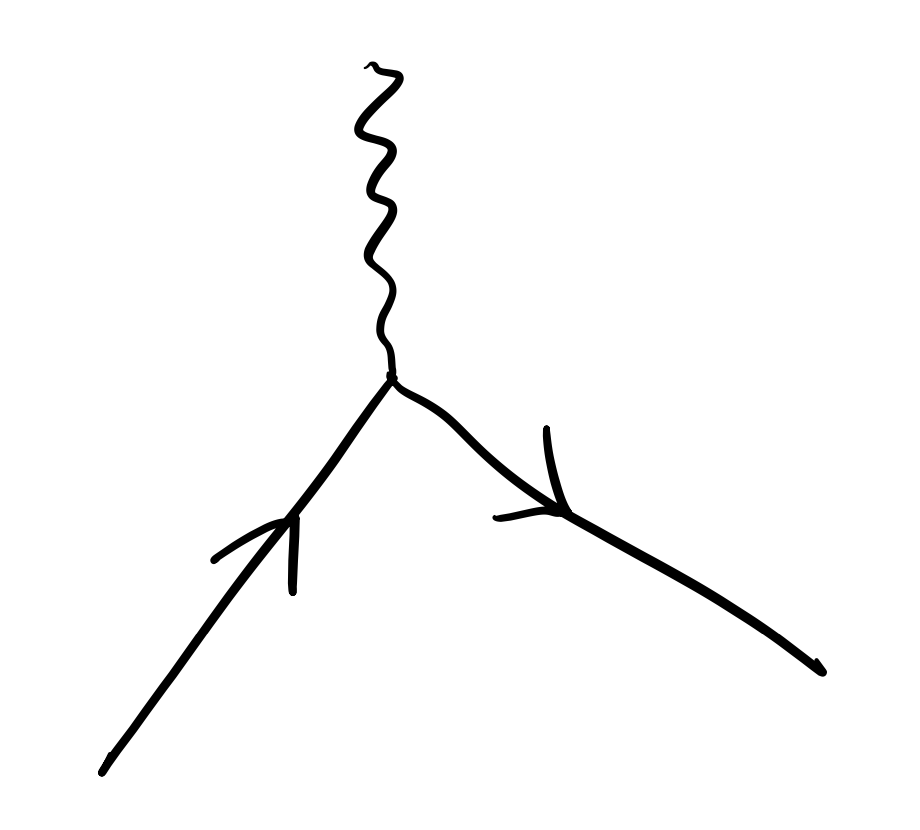
\includegraphics[scale=0.35]{Lectures/Images/lec9-diagram.png}
\end{center}

Let us first compute it in the free theory, using Wick contractions:
\begin{equation}
    \avg{j^\mu(x) \psi(y)\bar{\psi}(0)} = \avg{\bar{\psi}(x)\gamma^\mu \psi(x)\psi(y)\bar{\psi}(0)}
\end{equation}
The only connected correlators come from pairing $\psi(y)$ with $\bar{\psi}(x)$ (moving this fermion observable to pair them requires two moves, so no overall negative sign) and $\psi(x)$ with $\bar{\psi}(0)$ and thus we obtain:
\begin{equation}
    \avg{j^\mu(x) \psi(y)\bar{\psi}(0)} = G(y-x)\gamma^\mu G(x)
\end{equation}
Let us Fourier transform this (as this is where the Green's functions look simple):
\begin{equation}
    \avg{j^\mu_p \psi_{p'}\bar{\psi}} = \int d^4x d^4y e^{-ipx}e^{-ip'y}G(y - x)\gamma^\mu G(x) \stackrel{y \to z = y-x}{\to} \int_{zx} e^{-ipx}e^{-ip'(z + x)}G(z)\gamma^\mu G(x) = G(p')\gamma^\mu G(p + p')
\end{equation}
So in the free theory our vertex function looks like:

\begin{center}
    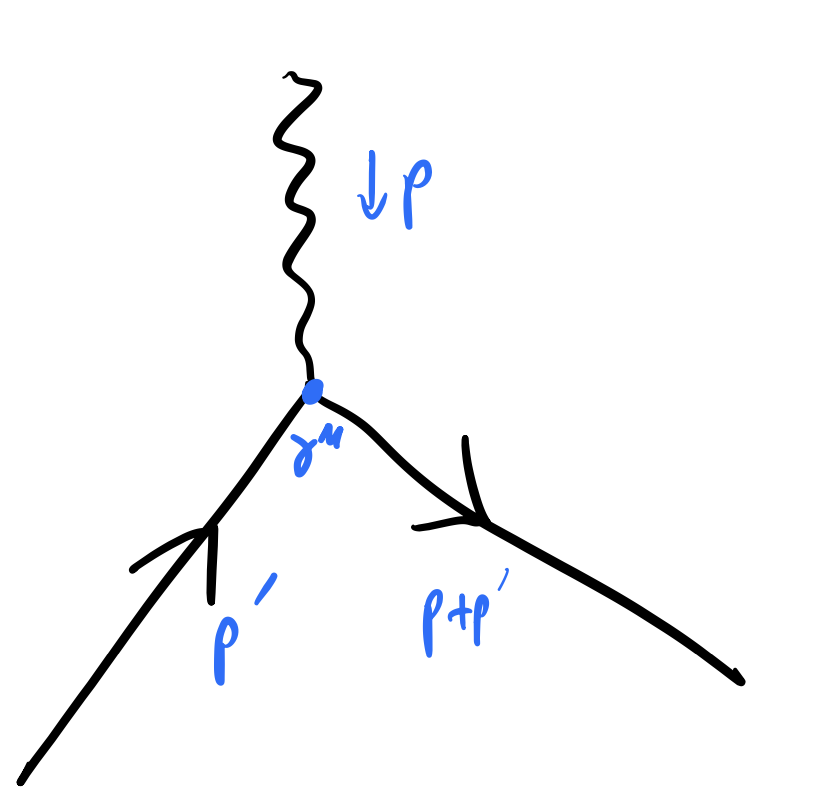
\includegraphics[scale=0.35]{Lectures/Images/lec9-free.png}
\end{center}

We can look at the ``amputated'' vertex, which will simply be obtained by multiplying the above by $G(p')^{-1} G(p+p')^{-1}$, which yields:
\begin{equation}
    \avg{j^\mu_p \psi_{p'}\bar{\psi}}_{\text{amp}} = \gamma^\mu
\end{equation}

So, we have the tree-level result. We are now interested in corrections to this answer. What kind of diagrams will give corrections to this vertex? At one loop we have three diagrams:

\begin{center}
    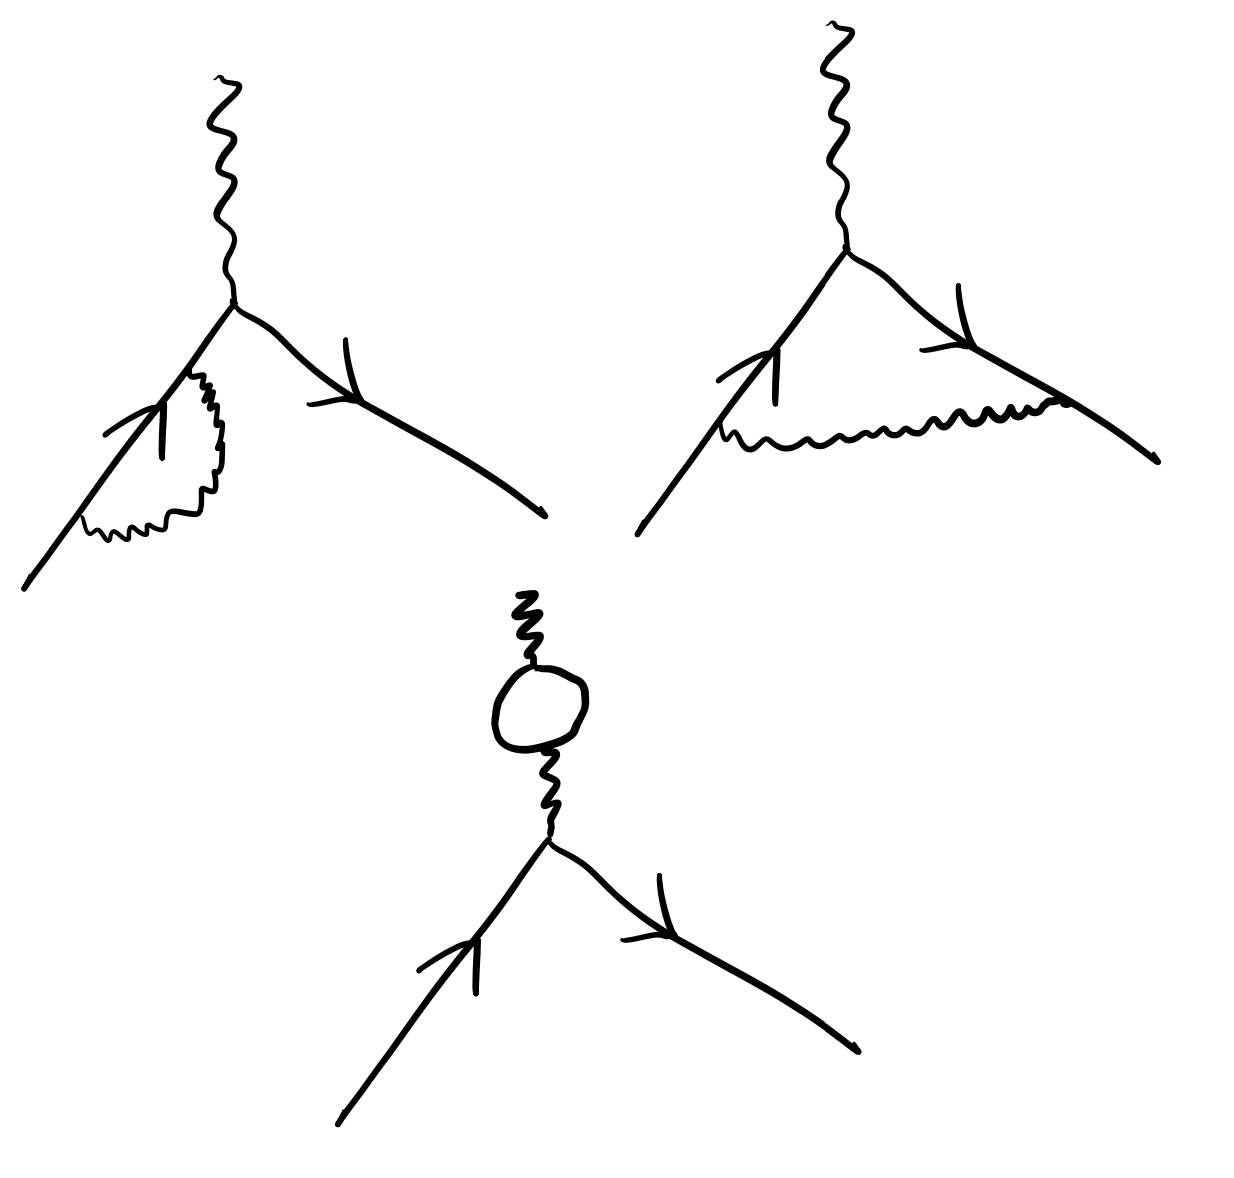
\includegraphics[scale=0.35]{Lectures/Images/lec9-oneloop.png}
\end{center}

In the interacting theory, the vertex function will take on a different form than the free theory. One can show that the most general form that it can take is:
\begin{equation}
    \avg{j^\mu_p \psi_{p'}\bar{\psi}}_{\text{amp}} = \gamma^\mu F_1(\frac{p^2}{m^2}) + iS^{\mu\nu}\frac{p_\nu}{m}F_2(\frac{p^2}{m^2}) 
\end{equation}
with:
\begin{equation}
    S^{\mu\nu} = \frac{i}{4}[\gamma^\mu, \gamma^\nu]
\end{equation}
In the free theory we had $F_1(\frac{p^2}{m^2}) = 1$ and $F_2(\frac{p^2}{m^2})  = 0$, but as we add corrections these functions will come alive. The $F_i$ are called ``form factors''. You can think about the above correlation function as probing the structure of the electron through:
\begin{equation}
    \avg{j^\mu_p\psi_{p'}\bar{\psi}} \sim \bra{p + p'}j^\mu \ket{p'}.
\end{equation}
Intuitively, the first term measures the renormalization of the charge $e$. The second term produces an ``anomalous'' electron dipole moment (which corrects for the classical prediction). How do we see this? One would get an $F_2$ contribution at tree level from a vertex:
\begin{equation}
    S_{\text{eff}} = \int \frac{a}{2m}F_{\mu\nu}\bar{\psi}S^{\mu\nu}\psi = -\int \frac{a}{m}\p_\nu A_\mu \bar{\psi}S^{\mu\nu}\psi
\end{equation}
with $\p_\nu A_\mu$ giving $ip_\nu$ and $a \sim F_2(0)$. Compare this with $A_\mu \bar{\psi}\gamma^\mu\psi$ which was our original vertex. Let's see how this term produces a dipole moment via studying the equation of motion:
\begin{equation}
    0 = \frac{\delta S}{\delta \bar{\psi}} = (i\slashed{D} - m + \frac{a}{2m}F_{\mu\nu}S^{\mu\nu})\psi
\end{equation} 
If we multiply this by the EOM with flipped sign:
\begin{equation}
    \begin{split}
        0 &= (i\slashed{D} + m - \frac{a}{2m}F_{\mu\nu}S^{\mu\nu})(i\slashed{D} - m + \frac{a}{2m}F_{\mu\nu}S^{\mu\nu})\psi 
        \\ &= (-\slashed{D}^2 - (m - \frac{a}{2m}F_{\mu\nu}S^{\mu\nu})^2)\psi
        \\ &\approx (-\slashed{D}^2 - m^2 + aF_{\mu\nu}S^{\mu\nu})\psi
        \\ &= (-D^2 - m^2 + (1 + a)F_{\mu\nu}S^{\mu\nu})\psi
    \end{split}
\end{equation}
Recall that $\slashed{D}^2 = D^2 - F_{\mu\nu}S^{\mu\nu}$, and this second term gave rise to the leading order electron dipole moment. So, the $a$ simply adds to this dipole moment, yielding:
\begin{equation}
    \mu = \frac{e}{2m}(1 + F_2(0))
\end{equation}
All of this to show that the new feature gives rise to the anomalous dipole moment.

Note that some qualities of the electron do not change via corrections (e.g. the number is protected) but others do (e.g. the dipole moment, for which we obtain small corrections in perturbation theory).

\subsection{Ward Identities for QED}
The vertex function is constrained by the Ward identity:
\begin{equation}
    \p_\mu \avg{j^\mu(x)\psi(y)\bar{\psi}(0)} = (\delta^4(x) - \delta^4(x-y))\avg{\psi(y)\bar{\psi}(0)}
\end{equation}
this is very useful as it relates the 4-point function to a 2-point function, and moreover, it holds non-perturbatively. Writing it in momentum space:
\begin{equation}
    -p_\mu \avg{j^\mu_p \psi_{p'}\bar{\psi}} = i[G(p') - G(p + p')]
\end{equation}
Thus, $p_\mu$ dotted with the four-point function just gives us the difference of two propagators (in the interacting theory, of course both sides of this equation become more complicated, but the identity still holds). Let's check this in the free theory as a consistency check. We consider the amputated versions here. On the LHS, we get $-\slashed{p}$, and on the RHS we have:
\begin{equation}
    \frac{1}{G(p')}i[G(p') - G(p + p')]\frac{1}{G(p+p')} = i\left(\frac{1}{G(p+p')} - \frac{1}{G(p')}\right) = i\left(\frac{\slashed{p} + \slashed{p}'}{-i} - \frac{\slashed{p}'}{-i}\right) = -\slashed{p}
\end{equation}
so the ward identity checks out.

\subsection{Proof of the form of the vertex function}
Let us call the fermion momenta $q_1$ and $q_2$. Using lorentz invariance we set $q_2 = -p - q_1$, and then we write down a general form:
\begin{equation}
    \avg{j^\mu_p \psi_{q_1}\bar{\psi}_{q_2}}_{\text{amp}} = q_1^\mu f_1 + q_2^\mu f_2 + f_3 \gamma^\mu f_4
\end{equation}
where the $f_i$ are matrices that depend only on lorentz covariant quantities:
\begin{equation}
    f_i(q_1^2, q_2^2, q_1\cdot q_2, \slashed{q}_1, \slashed{q}_2)
\end{equation}
This is a bit of a mess, it depends on too many parameters. To start, we put the fermions on shell $q_1^2 = q_2^2 = -m^2$. We will further sandwich it with spinors for which $(\slashed{p} + m)u(p) = 0$, these are precisely the spinors that we obtained when solving the Dirac equation, so sandwiching the above with $\bar{u}(q_1)\ldots u(q_2)$:
\begin{equation}
    \bar{u}(q_1)\avg{j^\mu_p \psi_{q_1}\bar{\psi}_{q_2}}u(q_2)
\end{equation}
this has a simple general form. Namely, we can move the $\slashed{q}_2$s to act them on the $u(q_2)$, giving $\slashed{q}_2u(q_2) = -mu(q_2)$ (and vise versa for $q_1$), which gives:
\begin{equation}
    \bar{u}(q_1)\avg{j^\mu_p \psi_{q_1}\bar{\psi}_{q_2}}u(q_2) = \bar{u}(q_1)(q_1^\mu f_1 + q_2^\mu f_2 + f_3\gamma^\mu)u(q_2)
\end{equation}
so we are down to three functions, and the $f_i$ are now just truly scalar functions rather than matrices, with $f_i = f_i(q_1 \cdot q_2)$. We are almost there, but we have three functions rather than the desired 2. Finally, we will use the fact that the vertex function must satisfy Ward identities, namely if we act on the above with $-p_\mu$ we get:
\begin{equation}
    \bar{u}(q_1)\left(\frac{1}{G(q_2)} - \frac{1}{G(q_1)}\right)u(q_2) = 0
\end{equation}
Which tells us that if we act on the vertex function with $p_\mu$ it must vanish, hence:
\begin{equation}
    0 = (p \cdot q_1 f_1 + p \cdot q_2 f_2)\bar{u}(q_1)u(q_2) + f_3\bar{u}(q_1)\slashed{p}u(q_2)
\end{equation}
The last term satisfies the Ward identity on its own; $\slashed{p} = -\slashed{q}_1 - \slashed{q}_2$, acting the two parts on the opposite sides, we find it vanishes:
\begin{equation}
    \bar{u}(q_1)(-\slashed{q}_1 - \slashed{q}_2)u(q_2) = \bar{u}(q_1)(-m + m)u(q_2) = 0
\end{equation}
Thus:
\begin{equation}
    0 = (q_1 + q_2)\cdot q_1f_1 + (q_1 + q_2)\cdot q_2 f_2 = (-2m^2+ 2q_1 \cdot q_2)(f_1 + f_2) \implies f_2 = -f_1
\end{equation}
where we have used $p^2 = (q_1 + q_2)^2 = -2m^2 + 2q_1 \cdot q_2$. And thus we only have two independent functions:
\begin{equation}
    \bar{u}(q_1)\avg{j^\mu_p \psi_{q_1}\bar{\psi}_{q_2}}u(q_2) = \bar{u}(q_1)\left(\gamma^\mu F_1(\frac{p^2}{m^2}) + (q_1^\mu - q_2^\mu)F_2(\frac{p^2}{m^2})\right)u(q_2)
\end{equation}
This is a very powerful statement because it is true non-perturbatively; it is always true!

On Thursday we continue the calculations by computing the corrections to the electron dipole moment at one loop.